\documentclass[11pt,a4paper]{report}
\usepackage[utf8]{inputenc}
\usepackage{authblk}
\usepackage{graphicx}
\usepackage{float}
\usepackage{color}
\usepackage{subcaption}
\usepackage{makeidx}
\usepackage{lmodern}
\usepackage{anyfontsize}
\usepackage[utf8]{inputenx}
\usepackage[T1]{fontenc}
\usepackage{amssymb}
\usepackage{amsmath}
\usepackage{setspace}
%\usepackage[legalpaper, landscape, margin=2in]{geometry}
%\usepackage{biblatex}
%\usepackage{chemfig}
\usepackage[left=5cm,right=3cm,top=4cm,bottom=4cm]{geometry}

\begin{document}	
	\begin{titlepage}
		\begin{center}
	\LARGE\textbf{ATOMIC
	NEURAL NETWORKS FOR \linebreak \linebreak
	PREDICTING MOLECULAR \linebreak \linebreak PROPERTIES}
	 \linebreak
	 \linebreak
\linebreak
\large \textit{A thesis submitted in partial fulfilment of the requirements \linebreak for the award of the degree of}
\linebreak
\linebreak
\LARGE \textsc{Integrated Master of Science in Physics}
\linebreak
\linebreak
	 \large \textit{Submitted by}
\linebreak
\linebreak
	 \LARGE \textsc{HemaPrasath V}
	 \linebreak
	 \linebreak
	 \large\upshape (Reg. No. I150117)
	 \linebreak
	 \linebreak
	 \large \itshape Under the guidance of
	 \linebreak
\linebreak
	 \large \upshape Dr. M. \textsc{Ponmurugan}
	\linebreak
	\linebreak
	\text{(Assistant Proffessor)}
\upshape\large
\begin{figure} [H]
	\centering
	
\includegraphics[width=0.3\textwidth]{C:/Users/hp/Desktop/thesis/cutn_logo.png}
\end{figure}
\textsc{Department of physics \linebreak
School of Basic and Apllied Sciences\linebreak
Central University of Tamil Nadu\linebreak
Thiruvarur \linebreak
May-2020}
	\end{center}
	\end{titlepage}
	
	\begin{center}
	\huge \bfseries Declaration
	
\end{center}
\pagenumbering{roman}
{\onehalfspacing I, HemaPrasath V, hereby declare that the project thesis, entitled \emph{``Atomic Neural Networks for predicting Molecular Properties''} which is submitted by me in partial fulfilment of the requirements for the award of the degree of \linebreak INTEGRATED MASTER OF SCIENCE in PHYSICS comprises only my original research work and due acknowledgement has been made in the text, is produced under the guidance of Dr. M. Ponmurugan, Assistant Professor, \linebreak Department of Physics, School of Basic and Applied Sciences, \linebreak Central University of Tamil Nadu, Thiruvarur.}
\\\\\\\\\\\\\\\\\\\\\\
Date:
\\
Place: Thiruvarur$~~~~~~~~~~~~~~~~~~~~~~~~~~~~~~~~~~~~~~~~~~~~~~~~~~~~~~~~~~~~~~~$      Signature of the Candidate \linebreak 
$~~~~~~~~~~~~~~~~~~~~~~~~~~~~~~~~~~~~~~~~~~~~~~~~~~~~~~~~~~~~~~~~~~~~~~~~$     (HemaPrasath.V)

\pagebreak
\begin{center}
	\begin{figure} [H]
		\begin{subfigure}{0.5\textwidth}
		\centering
		
\includegraphics[width=1.6\textwidth]{C:/Users/hp/Desktop/thesis/cutn_logo2.png}
		\end{subfigure}%
		\begin{subfigure}{0.8\textwidth}
		\centering
		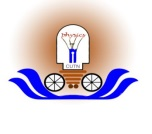
\includegraphics[width=0.2\linewidth]{C:/Users/hp/Desktop/thesis/phy_logo.png}
		\end{subfigure}
	\end{figure}

\underline {\scshape\bfseries\large CERTIFICATE}
\end{center}
\large {This is to certify that this project entitled {\bfseries \normalsize``ATOMIC NEURAL NETWORKS FOR PREDICTING MOLECULAR PROPERTIES''} submitted in partial fulfilment for the requirements for the award of the degree of {\normalsize\bfseries \scshape INTEGRATED MASTER OF  SCIENCE  } in {\normalsize\bfseries \scshape PHYSICS} to the Central University of Tamil Nadu, done by 
 {\normalsize\bfseries \scshape Mr. HEMAPRASATH V}, Roll No. I150117 is an authentic work carried out by him at \linebreak {\itshape Department of Physics, Central University of Tamil Nadu} under my guidance . The matter embodied in this project work has not been submitted earlier for award of any degree or diploma to the best of my knowledge and belief.
 \\
 \\\\\\\\\\
 Date: $~~~~~~~~~~~~~~~~~~~~~~~~~~~~~~~~~~~~~~~~~~~~~~~~~~~~~~~~$ Dr.$~~$M.$~~$Ponmurugan
 \\
 Place: Thiruvarur $~~~~~~~~~~~~~~~~~~~~~~~~~~~~~~~~~~~~~~~~~~~$Project Supervisor
 \\
 \\
 \\\\\\\\
 Head of the Department $~~~~~~~~~~~~~~~~~~~~~~~$ Project Co-ordinator
\pagebreak


{\onehalfspacing
		
	{\centering \bfseries \LARGE Acknowledgement}
\\\\	
$~~~~~~$I would like to express my gratitude to my supervisor \linebreak
Dr. M. Ponmurugan, Assistant Professor, Department of Physics, Central University of TamilNadu for the useful comments and all the support, motivation and encouragement he has given me throughout my project period. I extend my gratitude to the Head of the Department, Prof. L. Kavitha and all the faculty members of the department. I would like to thank the Ph.D students who worked in the same lab as me and my classmates for their advice and good intent along this work. I also thank my parents who have been in this through thick and thin with me.}
\pagebreak
	\begin{center}
	\section*{Abstract}
	\end{center}
Atomic Neural Networks (ANNs) constitute a class of machine learning models establishing Quantitative structure-activity relationships (QSARs), structure-property relationships in molecules. PiNN, a Python library was developed for implementing interpretable ANN Architectures and existing architectures efficiently. It also offers built-in dataset loaders for ease of access for different formats of molecular data, custom ANN designs and model types. Molecular property is regressed against other molecular information using Machine Learning techniques. Here, Dipole moment is regressed against the structure of certain organic molecules, building a dipole model for predicton. The dipole model's accuracy is compared for different sample sizes of the number of organic molecules used for regression.
	
\

	{\tableofcontents}
	\listoffigures
	
\chapter{Machine Learning Techniques}
\pagenumbering{arabic}
\section{Introduction}
	
	\large
	
	One of the many Machine Learning techniques is to map a relation between information by inference without any explicit instructions. In many fields of science, mapping between informations can be used to establish relationship that help build an approximate function that in turn help build models to study further. As an Example, a function $f:\left\{x_i, Z_i\right\}\,\to\,P$ is used to map the structure of a molecule or a material to its property $P$, where $\left\{x_i, Z_i\right\}$ represent the structural information of the molecule/material. In Conventional methods, if $P$ is the total energy, then approximate solutions to the Schr{\"o}dinger equation\cite{QM} is found using traditional computational methods that are resource-intensive and available commercially even with today's better computational resources. 

Machine Learning techniques recognise patterns from pre-existing information (from a database) to properly build functions that properly map relations to the property. This mapping function is then used to predict for new structures. The general task in machine learning is to determine what patterns to recognise from the database; to build the functions that map relations with ease and computational efficiency.

\section{Neural Networks} \label{NN}
\large
	Simple Neural Networks are directed 'graphs' of simulated nodes. A 'graph' consists of nodes and edges that connect them. The Neural Networks are inspired as a biological neuron. The nodes that connect to another node is one-directional i.e., the node that sends information to another node does not receive from the same. The nodes which connect to the next node belong to a single layer in the neural network. Each layer that sends information performs an operation on the information. The Neural Network Architecture refers to the number of layers, number of nodes in each of those layers, operation for each layer. 
\begin{figure} [H]
\centering
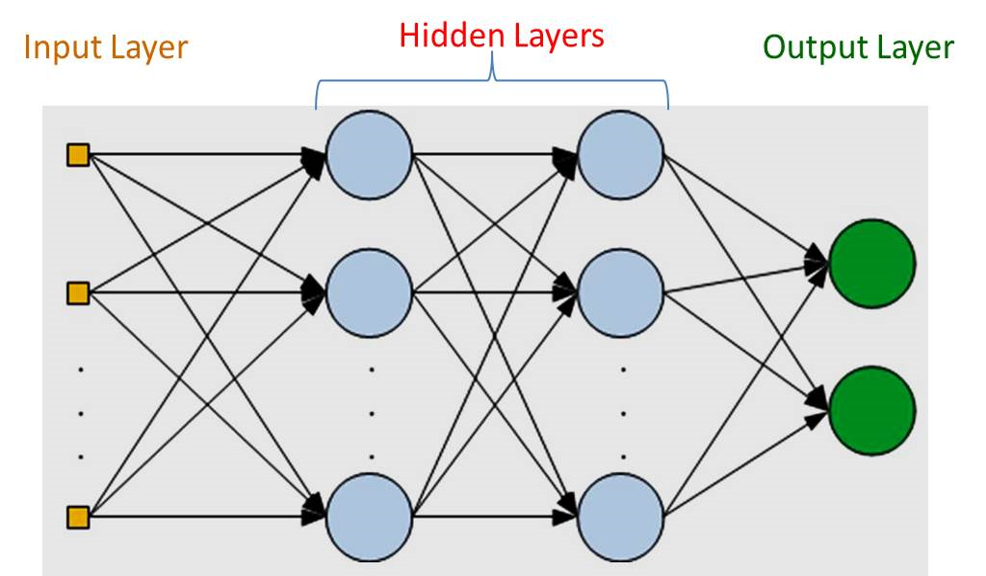
\includegraphics[width=0.75\textwidth]{C:/Users/hp/Desktop/thesis/NN_Arch.png}
\caption{A Simplified Neural Network Architecture}
\end{figure}

Edges determine the weight of the connection between the nodes that connect them. The Hidden Layers operate on the information sent from the previous layer using a set of activation functions. Mathematially, if the inputs are $a_1,a_2,...,a_n$ and the weights are $w_1,w_2,...,w_n$, then the value output for a single node would be:
\begin{equation} 
a^j=f( b+ \sum_{i=1}^{n}{a_i^{j-1}*w_i^{j-1}} )
\end{equation}
where $f$ is the activation function of choice, $b$ is the bias, $a^j$ refers to the nodes in the $j^{th}$ layer. Each $a_i^{j-1}$ refers to the values of the previous layer and $w_i$, the weight between the nodes connecting the previous layer. Thus the output layer gives a combined value of all the hidden layers, depending on the weighted connections between nodes and the bias value $b$. Thus, the value of the output node will be:
\begin{equation} \label{eq:1}
y=f( b+ \sum_{i=1}^{n}{a_i^{j}*w_i^{j}})
\end{equation}
The 'learning' aspect using pre-existing information takes place here. As the output value is determined by the bias $b$ and weights between each nodes of every layers $w^{j}_i$, a cost function is introduced that gives us the error between the Neural network predicted value and the value from the database. Hence, it is necessary for the database to contain both the information that is used to predict and the predicted value to build a model. The cost function is of choice and depends on the model that is built. The cost function is then used to modify the weight values from Eq. \ref{eq:1}. 

The modification of the weight values are such that the cost function $reduces$ over many iterations of the neural network through a huge database for generality. This is done by another operation using optimizers. A common optimizer operation is a stochastic gradient descent which finds the global minima for the cost function and the multiple weight values. Other optimizers can also be used depending on the complexity of the model and the efficiency required. A single best type of optimizer/activation functions cannot be used, as different optimizers fit in better for different models.

Certain hyperparameters are pre-defined before building a model that helps make the learning process efficient and accurate such as the activation functions, the learning rate and the architecture of the neural network itself. The learning rate specifies the rate at which the global minima of the cost function w.r.to the learnable parameters (weights and biases) is approached. 

Machine Learning models contain various techniques for prediction, classification or recognizing patterns/trends\cite{ML}. Of which the above technique is a generic technique of using existing database of information from both the predictor and prediction, usually called the values and its labels i.e., each value is mapped to its label value. This mode of operation is called the supervised learning.

From this chapter, the concept of Machine Learning and its potential for predicting regressions and recognising patterns is introduced. The technique of supervised learning using pre-existing database of information for building prediction models of choice is understood. It is also understood that the machine learning techniques can be used to increase efficiency.


\chapter{Atomic Neural Networks} \label{chap_ANN}
\section{Introduction} \label{ANN}
\large

Atomic Neural Networks (ANNs) are a class of machine learning models that help predict physico-chemical properties of molecules and materials. As mentioned before in \ref{NN}, ANNs usually use supervised learning techniques. More advanced NN architectures are prepared for accuracy based off on this technique. The existing database for ANN models are collected from pre-existing information that are calculated by traditional methods. 

\begin{figure} [H]
\centering
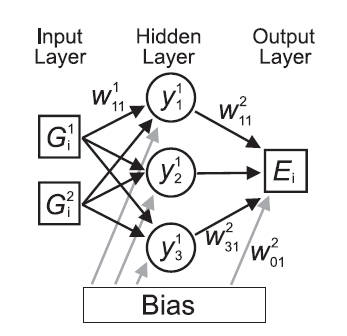
\includegraphics[width=0.5 \textwidth]{C:/Users/hp/Desktop/thesis/Sim_ANN.png}
\caption{Example of a simple ANN model that predicts the energy $E_i$ of a configuration $i$ using the generalized coordinates $G^1_i, G^2_i$. }
\end{figure}

The node in the output layer yields the energy $E_i$ of the configuration $i$ depending on the generalized coordinates $G^1_i$ and $G^2_i$. The hidden layers connect the input and the output layer with a specified number of nodes. These nodes are connected by the weights between the nodes, which are real-valued and are chosen randomly, initially. For the example, the output of the energy configuration is given by the expression:
\begin{equation} 
E_i=f^2_a[w_{01}^2+\sum_{j=1}^{3}{w^2_{j1}f^1_a(w^1_{0j}+\sum_{\mu=1}^{2}{w^1_{\mu j}G^{\mu}_i)}}]
\end{equation}
The weights $w^k_{ij}$ and the bias weight $w^k_{0j}$ which are initially randomly chosen, does not correspond to the correct total energy output. Hence, to adjust these learnable parameters for proper prediction, the known total energies for a known set of configurations are used to optimize the set of these parameters, a cost function is constructed to minimize the error in an iterative way. The optimized set of 'learned' parameters can then be used to calculate the energy for a new set of coordinates.

Although this approach is novel\cite{simANN}, there are disadvantages associated with this setup. Namely, the coordinates of the configuration is fixed (number of degrees of freedom) and cannot be applied for higher set of coordinates as the optimized set of weights are vallid only for a specified size. Also, the weights of the NN are different for each configuration, meaning NN is not arbitrary towards similar configurations, allowing to predict falsely. 

In general, the ANN models can be made to predict with greater accuracy and hence more efficiently. This means that the ANN model must preserve translational, rotational and even permutational invariance across different configurations of the system used to predict.

\section{Generalized Atomic Neural Networks}
Another ANN topology is introduced that addresses the challenges mentioned in \ref{ANN}. Generalized Atomic Neural Networks\cite{BPNN} were introduced that considers different system sizes and invariance in different configurations. The idea of empirical potentials of the total energy $E$ of a configuration being represented as a sum of the atomic contrbutions $E_i$. \begin{equation} \label{em_en}
E=\sum_{i}{E_i}
\end{equation}
From the input layer to the second hidden layer, the cartesian coordinates $\left\{R^{\alpha}_i\right\}$ or any form of coordinates that specify structural configuration of a system are transformed to a set of symmetry function values $\left\{G^{\mu}_i\right\}$. These symmetry functions represent the energetically relevant local environment of each atom $i$ and are subsequently used for the input for the ANN. These function values depend on the positions of all the atoms in a system, shown by the dotted lines in Figure \ref{BPNN}
\begin{figure}  [H] 
\centering
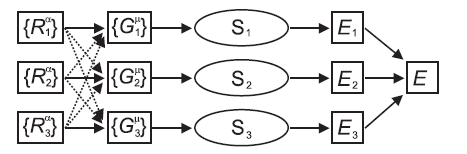
\includegraphics[width=0.75\textwidth]{C:/Users/hp/Desktop/thesis/BPNN.png}
\caption{Structure of a Generalized Neural Network to a system containing three atoms}
\label{BPNN} 
\end{figure}
For each atom $i$ in the system there is now a 'simple' ANN as mentioned in \ref{ANN}, which is called a subnet $S_i$ and which after the optimization of the weights yields the energy contribution $E_i$ of an atom in the system. Summing these energy contributions then finally yields the total energy of the system. To ensure the invariance of the total energy with respect to similar configurations of the system, the values of the weight parameters are constrained to be identical in each $S_i$ of such system. 

\subsection{Symmetry and cut-off Functions}
Radial Symmetry functions are constructed as a sum of Gaussians with the parameters $\eta$ and $R_s$, 
\begin{equation} \label{rad_sym}
G^1_i=\sum_{j\neq i}^{all}{e^{-\eta(R_{ij}-R_s)^2} f_c(R_{ij})} 
\end{equation}
Here, the symmetry function is set such that it is rotationally, translationally and permutationally invariant. Also, the number of symmetry functions is independent of the coordination number of an atom in the system, this is ensured by the summation over all the neighbours $j$ for the atom $i$. The value of the Radial symmetry function depends on these parameters $\eta$, $R_s$ and a cutoff function $f_c(R_{ij})$. 
\begin{equation} \label{cutoff}
f_c(R_{ij})=
\begin{cases} 
0.5 \times \Big[\cos \Big(\frac{\pi R_{ij}}{R_c}\Big)+1\Big] & \text{for} R_{ij} \leq R_c\\
0 & \text{for} R_{ij} > R_c\\
\end{cases}
\end{equation}
At interatomic distances $R_{ij}$ larger than the cutoff radius $R_c$, this cutoff-function yields zero value and slope. The cutoff $R_c$ has to be sufficiently large to include several nearest neighbours. This cutoff function helps determine the energetically relevant local environment for an atom $i$ in the system.

Angular symmetry functions are constructed for all triplets of atoms by summing the cosine values of the angles $\theta_{ijk} = \frac{\mathbf {R_{ij} \cdot R_{ik}} \\}{R_{ij}R_{ik}}$ centered at atom $i$, with $\mathbf{R_{ij}=R_i-R_j}\\$.
\begin{equation} \label{ang_sym}
G^2_i=2^{1-\zeta}\sum_{j,k \ne i}^{all}{(1+\lambda\cos{\theta_{ijk}})^{\zeta} } \times e^{-\eta(R^2_{ij}+R^2_{jk}+R^2_{ik})} f_c(R_{ij})f_c(R_{jk})f_c(R_{ik}),
\end{equation}
with the parameters $\lambda$ (=+1,-1), $\eta$ and $\zeta$. The multiplication by the three cutoff-functions and by the Gaussian gives a smooth decay to zero incase of large interatomic seperations. The use of symmetry functions and parameters is not unique, and many types of functions can be used to describe the suitable environment of an atom $i$.

In Conclusion, this generalized ANN architecture can be used to build models to predict for various system sizes and they provide with more accuracy, as the total energy is partitioned into effective atomic contributions\cite{BPNN} (Eq. \ref{em_en}). 

Hence, this ANN describes the local chemical environment of each atom (also called the fingerprint of the atomic environment\cite{atmfing}) using the set of symmetry functions from Eqs. \ref{rad_sym} and \ref{ang_sym}. This is generally called the Behler - Pahrinello Neural Network or the BPNN and has been succesfull for a wide-range of molecules and materials.

\section{Graph Convolutional Atomic Neural Networks}
In the field of Deep Learning is one of the most successful end-to-end techniques, Convolutional Neural Networks. The convolution in an NN, helps learn features (in terms of a simple ANN, the optimized set of weights) by creating a feature hierarchy.  For Graph Convolutional Neural Networks (GCNN) in atomic systems, the molecules and materials can be viewed as fully connected graphs\cite{GCNN}.

 A graph neural network considers an atom as nodes and their pairwise-interactions as edges of a graph. These pairwise interactions are are weighted edges that define the interaction features between the atoms connecting them. The essence of a Convolution, gathers information for each atom from their neighbouring atoms within a cut-off radius $R_c$ and creates a feature hierarchy. Node and edge feature vectors are updated through a function. 

This way the features are learned automatically, instead of manually hand-crafting them. Hierarchical atomic features\cite{fthier} are obtained by applying multi-stage concatenated convolution operations through a neural message passing function. By construction, the generation of the node features includes the element-specificity. Hence, GCNN has the same subnet for each element. This also proves effective performance for a variety of systems, also retaining invariance properties.
\begin{figure} [H]
\centering
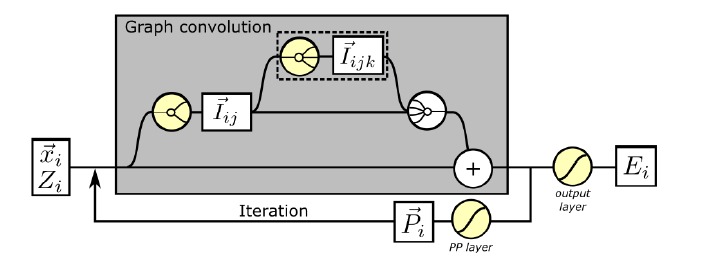
\includegraphics[width=0.75 \textwidth]{C:/Users/hp/Desktop/thesis/GCNN.png}
\caption{Representation of a GCNN framework in atomic systems}
\label{GCNN}
\end{figure}
In Fig. \ref{GCNN}, the input matrices $\vec{x}_i$ and $Z_i$ provide the structural information of a system. The $\vec{I}_{ij}$ and $\vec{I}_{ijk}$ represent the pairwise and the triplewise interactions caused by the radial and the angular terms respectively. The Graph Convolution block (black box) is the convolution filter that creates a feature hierarchy iteratively updating the node and edge feature vectors.

This chapter introduces the concept of Atomic Neural Networks and its evolution with developments in the machine learning. It also shows the increased computational efficiency and accuracy achieved using these techniques, with accessible computational resources. 

The ANN helps predict properties from the structural information as $f:\left\{x_i, Z_i\right\}\,\to\,P$ stated. The Generalized ANN partakes this concept to partition effective atomic contributions of these properties and introduces symmetry functions to build prediction models for various system sizes and ensure rotational, translational and permutational invariance. The Graph Convolutional NNs considers the molecular systems as undirected graphs and creates hierarchical features to learn pairwise interactions between atoms as atomic fingerprints\cite{atmfing}. These different variations help create sophisticated systems for building prediction models of various molecular system properties which in turn can be used to build physical models.


\chapter{PiNN Python Package for ANN}

\section{Introduction}
Implementing Atomic Neural Networks through computational systems is the next step in the process of building the aforementioned NN models in \ref{chap_ANN}. The computer code for the building of models can be done through multiple channels, and the choice is dependent on factors like the ease of computational coding in different platforms, complexity of the model that is required to build, or the freedom to implement wide-variety of systems. 
Each coding platform offers different features and the choosing of one platform does not mean that the one is a better. 

The PiNN library\cite{PiNN} is implemented in Python to make the building of ANNs interpretable and implementing with comptuational ease efficiently. Hence, to promote the application of ANNs in the scientific communities, PiNN is a reliable, general-purpose, open-source-code.

Here, we use PiNN, a library in the Python coding platform for computational ease and also for building a variety of systems using the PiNN - Python Library. The code for the library is not implemented in the Python  and is an external code distributed under a permisive BSD license and is freely accessible at https://github.com/Teoroo-CMC/PiNN/ with full documentation and tutorials.


\section{Using the PiNN - Python Package}
The PiNN library is built on top of the TensorFlow\cite{tf} by Google, which is generally used to implement machine learning and deep-learning models for general purposes. The TensorFlow library offers to use the Graphical Processing Units (GPUs) of computer systems for computational power. PiNN offers modularization of existing models (as discussed in \ref{chap_ANN}), which can be re-used for different uses. To reduce difficulty of the training tasks, customized dataset loaders are in-built within the library.
Also, it has in-built physical models that can be built for prediction of certain properties.

Building of an ANN can be split into three stages and the PiNN modules consist of three modules in par to this:
\begin{itemize}
\item
input/output (io) module for Preparing the datasets (as inputs for the ANN from various formats of data) 
\item
Networks module for defining the ANN architecture (with the different layers and different nodes for each of these layers and their functions, also the final cost functions and optimization technique choices)
\item
Models for model defnition (to predict the required property that is regressed from the structural information)
\end{itemize}
\begin{figure}
\centering 
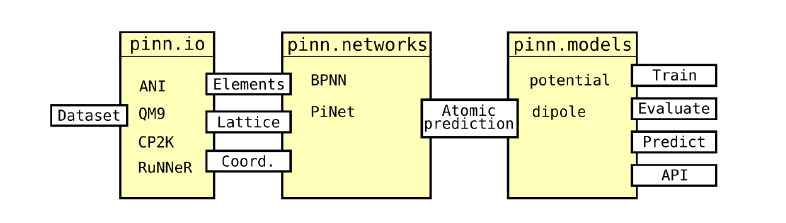
\includegraphics[width=1.05\textwidth]{C:/Users/hp/Desktop/thesis/modules.png}
\caption{Illustration of a structure of an ANN using the PiNN library}
\end{figure}

The Modularization of networks can be done without touching the internal Python code base. This design enables to easily import an arbitrary dataset within the ANN. 

One can also implement new ANN architectures from scratch in the "networks" module and use the other modules with code ease. Similarly, the "models" module could be extended to build for different property predictions with the same existing ANN architectures or to interface with external codes.

\subsection{Pairwise Interaction and Interaction Pooling} \label{PI and IP}
In PiNN, both the BPNN and GCNN is defined with two important abstractions : The Pairwise Interaction (PI) and Interaction Pooling (IP) operations. Labelling each atom in the system with $i$ and its atomic property $\vec{P_i}$, the PI is expressed as a function of the intial atomic properties of two atoms and their distance,
\begin{equation} \label{PI}
\vec{I_{ij}^t}=PI(\vec{P_i^t},\vec{P_j^t},r_{ij})
\end{equation}
where t is an iterator. For BPNN, $t=0$ and for GCNN, $t+1$ is the number of Graph Convolution (GC) blocks.

The IP is in contrast to the PI operation, where the pairwise interactions associated with the atom $i$ generate the atomic property. This is done by passing all the pairwise interactions of the atom $i$ and summing them to another function. The summation ensures permuational invariance of the generated atomic property.
\begin{equation} \label{IP}
\vec{P_i^{t+1}}=IP\bigg(\sum_{j}{\vec{I_{ij}^t}}\bigg)
\end{equation}

The combination of the PI and IP operations used generates an updated atomic property through $t+1$ iterations of GC blocks, with information collected from neighbouring atoms. This is referred to as the atomic fingerprint or a neural message passing function\cite{msg}. Through the iterations of GC blocks $PI+IP \rightarrow PI+IP,..., \vec{I_{ij}}$ also gets updated. Although the actual forms of PI and IP operations differ from the mentioned, the abstraction remains, allowing to create different functions for novel ANN architectures.

\section{PiNet - A GCNN variant of an ANN}
The feature of PiNN that allows modularization of any existing ANN architecture is greatly exploited, as the library offers its own custom GCNN variant of an ANN architecture, allowing for interpretation of the ANN activations. The PiNet\cite{PiNN} uses GC blocks to iteratively update molecular features. The PiNet can be used for various other model definitions apart from the in-built models - Potential and Dipole models.

\subsection{Architecture}
In PiNet, the PI is defined as a function of distance between both the interacting atoms, affecting the atomic property in turn. The weight matrix $\mathbf{W_{ij}}\\$ depends on both atomic properties $\vec{P_i}$ and $\vec{P_j}$. This weight matrix generates the PI value $\vec{I_{ij}}$. The advantage of the weight matrix is to have different radial dependence for each component of 
$\vec{I_{ij}}$, which is unique to PiNet.
\begin{equation}
\mathbf{W_{ij}}\\=NN^{PI-Layer}([\vec{P_i},\vec{P_j}])
\end{equation}
where NN is a feed-forward neural layer generating the weight matrix from the atomic properties of the interacting atoms.
Expressing the interatomic distances through a radial symmetry function, $e_{ij}$ (From Eq. \ref{rad_sym}):
\begin{equation}
\vec{e_{ij}}=f_c(r_{ij}) \cdot [e^{-\eta(r_{ij}-r_1)^2}, e^{-\eta(r_{ij}-r_2)^2},\ldots]
\end{equation}
where the cutoff function is from the Eq.\ref{cutoff} ensuring the interaction and its slope vanish at the cutoff radius $R_c$. The centers of the Gaussian functions $r_1,r_2,\ldots,r_{n_{basis}}$ are chosen to be evenly spaced between 0 and $R_c$, and the $\eta$ determines the width of the Gaussians. Although, the freedom to integrate other cutoff functions are possible, the default cutoff function is set to this equation.

\begin{figure} 
\centering
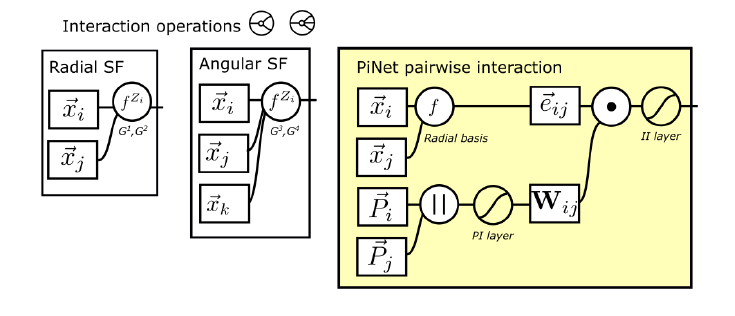
\includegraphics[width=0.85\textwidth]{C:/Users/hp/Desktop/thesis/PI.png}
\caption{Illustration showing the Pairwise Interaction Operation in a PiNet}
\label{PI}
\end{figure}
Then, the activation through the II layer (namely Interaction-to-Interaction), generates using another feed-forward NN using the information from the radial basis $\vec{e_{ij}}$ and the weight matrix $\mathbf{W_{ij}}\\$.
\begin{equation}
\vec{I_{ij}}=NN^{II-Layer}(\mathbf{W_{ij}}\\ \vec{e_{ij}})
\end{equation}
This process of generating the PI operation makes PiNet unique in contrast to other approaches where the interaction is directly generated from the distance and the atomic properties. It is to be noted that, despite not including a triplewise interaction part, the angular information is captured through the multiple iterations of the GC block.

After the PI Layer and the II Layer, the updated atomic property is calculated from all the pairwise interactions $\vec{I_{ij}}$ as part of the IP operation (As per Eq. \ref{IP}) through another feed-forward NN layer. And for further refinement of the atomic property, another PP (Property-to-Property) feed-forward NN layer is passed. In this approach, each feed-forward NN layer has its own unique activation functions. After multiple iterations through the GC block, the output layer is then used for optimization of the final set of weights to minimize errors.
\begin{figure} [H]
\centering
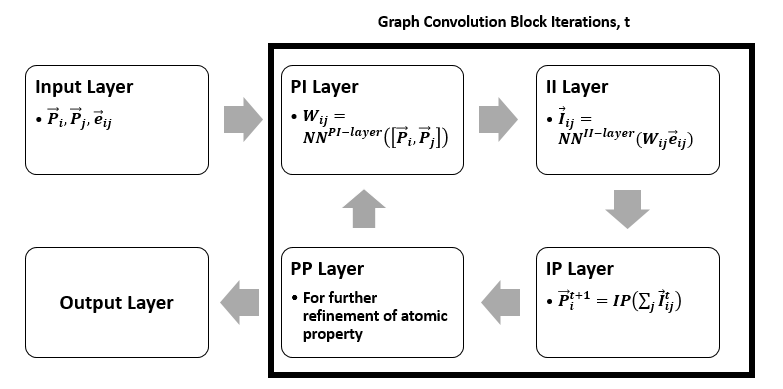
\includegraphics[width=0.95\textwidth]{C:/Users/hp/Desktop/thesis/PiNet.png}
\caption{Schematic Representation of a basic PiNet Architecture}
\label{PiNet}
\end{figure}

\section{Building a Dipole model using PiNet}
As an example of property predictions, PiNet ANN Architecture is used to regress the molecular dipole moment and partial charges,  accordingly,
\begin{equation} \label{dipoleeq}
\mu=\Bigg|\sum_{i=1}^{N}{\tilde{q_i}\vec{r_i}}\Bigg|
\end{equation}
where $\tilde{q_i}$ is the predicted partial charge on atom $i$ and the molecular dipole moment is acquired from a database. PiNN library offers for computational efficiency and ease. The property prediction is done in accordance to improve computational efficiency with limited power and resources. The aim is to predict values with higher accuracy using only these limited resources. 

Hence, multiple ANN model predictors are trained based on the corresponding computational resources the training model requires, ranging from highly accurate models (requiring higher computational power and time) to low accurate models (hence, only requiring lower computational time and power). 

\subsection{QM9 Dataset}
\begin{table} [H]
\centering
\begin{tabular}{c|c|c|c}
\hline
No. & Property & Description & Unit \\ [0.5ex]
\hline
1 & tag & 'gdb9' string to facilitate extraction & $\textthreequartersemdash$ \\
2 & $i$ & Consecutive, 1-based integer identifier & $\textthreequartersemdash$ \\
3 & $A$ & Rotational Constant & GHz \\
4 & $B$ & Rotational Constant & GHz \\
5 & $C$ & Rotational Constant & GHz \\
6 & $\mu$ & Dipole moment & D \\
7 & $\alpha$ & Isotropic Polarizability & $a_0^3$ \\
8 & $\epsilon_{HUMO}$ & Energy of HUMO & Ha \\
9 & $\epsilon_{LUMO}$ & Energy of LUMO & Ha \\
10 & $\epsilon_{gap}$ & Gap($\epsilon_{LUMO}$-$\epsilon_{HUMO}$) & Ha \\
11 & $\langle R^2 \rangle$ & Electronic spatial extent & $a^2_0$ \\
12 & zpve & Zero point vibrational energy & Ha \\
13 & $U_0$ & Internal Energy at 0 K & Ha \\
14 & $U$ & Internal Energy at 298.15 K & Ha \\
15 & $H$ & Enthalpy at 298.15 K & Ha \\
16 & $G$ & Free Energy at 298.15 K & Ha \\
17 & $C_v$ & Heat capacity at 298.15 K & Cal/mol.K \\
\hline
\end{tabular}
\caption{List of properties reported in a QM9 dataset for molecules}
\label{QM9}
\end{table}
The QM9 dataset\cite{QM9} is a database made of 134,000 small organic molecules containing computed geometric, electronic, energetic and thermodynamic properties at B3LYP/6-31G(2df,p) level of theory\cite{DFT}, is a highly recommended for benchmarking ANNs. The organic molecules are composed of all molecules of upto 9 heavy atoms. 

Other informations about the properties (listed in the Table \ref{QM9}) are also reported in this dataset for their corresponding organic molecules. The Table \ref{QM9} is in the format provided from the dataset.

\subsection{Benchmarks}
The Dipole model in-built with PiNN is used with constraint terms that ensure partial charges of each of the organic molecule to be zero. For building model variants based on computational power used, models with varying number of training data is used i.e., each model is built with random QM9 molecules with varying sample sizes. The $N$ number of molecules used for training and testing are: 

[10,50,100,200,500,1000,1500,2000,4000,5000,6500,8500,10000]. A total of 13 dipole models are built. Each model uses the same hyperparameters (listed in \ref{hyparam})
\begin{table} [H]
\centering
\begin{tabular}{c|c}
\hline
Hyperparameter & Value\\ [0.5ex]
\hline
PI Layer & [64]$\times$ 10 \\
II Layer & [64,64,64,64] \\
PP Layer & [64,64,64,64] \\
Output Layer & [64,1] \\
$R_c$ & 4.5 $\AA$ \\
Basis & Gaussian \\
GC blocks & 5 \\
$\eta$ & 3.0 $\AA^{-2}$ \\
$\eta_{basis}$ & 10 \\
Activation (each layer) & Hyperbolic Tangent \\
Learning rate & 3.0 $\times 10^{-4}$ \\
Training Steps & 10000 \\
\end{tabular}
\caption{Hyperparameters used for Dipole model building with N molecules}
\label{hyparam}
\end{table}
The QM9 molecular samples are split into training set and validation set with a ratio of 80:20, and the training samples are split into mini-batches with the following condition:
\begin{equation}
mini-batch-size =
\begin{cases}
 N & \text{for N $\leq$ 100} \\ 
100 & \text{for N $>$ 100} \\ 
\end{cases} 
\end{equation}
As the Number of molecules used for training for comparing accuracies, the cutoff and the radial basis functions are defaulted (\ref{PI and IP}).

\section{Results and Discussions}
The Dipole models built provided with reasonable accuracy, with increase in number of molecules, the error in the molecular dipole moment $\mu$ is minimized. The accuracy is compared using the validation split of the QM9 dataset in each model. Since, PiNN is built on top of the TensorFlow\cite{tf} Framework, the Tensorboard utility is used to visualize the training of the dipole model built for each sample size.

The decreasing trend seems to follow a logarithmic trendline, as the decrease in error for each model as the training size is increased, i.e., the accuracy of the model is more or less the same for even a significant increase in the training size (for larger training sizes). 

The error function that the building of the model is trained using the Mean Absolute Error (MAE), whereby the molecular dipole moment error $\mu_{MAE}$ is calculated as:
\begin{equation}
\mu_{MAE}=\big|\mu_{predicted} - \mu_{database}\big|
\end{equation}
Similarly, using the dipole moment prediction, the value of the partial charges, $\tilde{q_i}$ are predicted using the Eq. \ref{dipoleeq}. Then, the error in the partial charges $\tilde{q}_{i_{MAE}}$ is given by:
\begin{equation}
\tilde{q}_{i_{MAE}}=\big|\tilde{q}_{i_{predicted}} - \tilde{q}_{i_{database}}\big|
\end{equation}

\pagebreak
\begin{figure} 
\centering
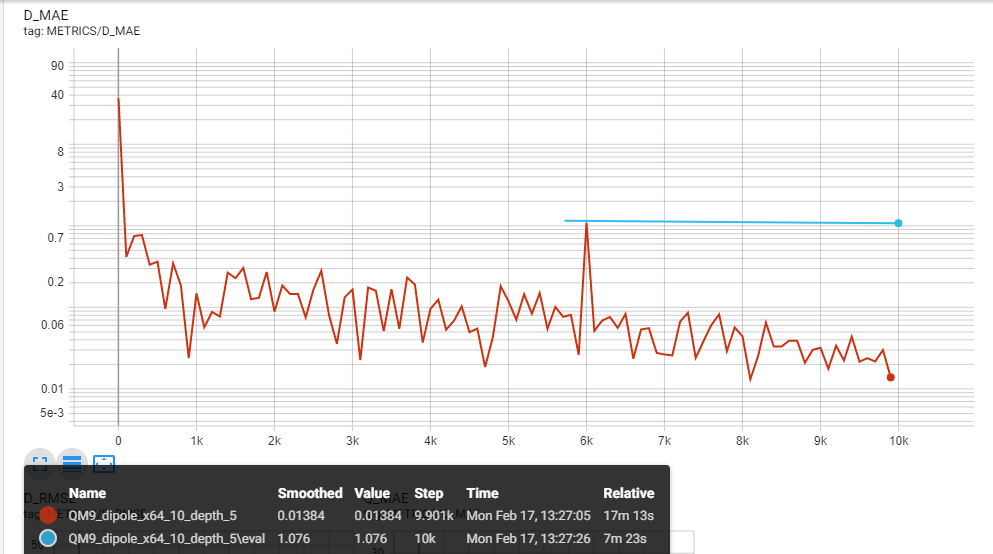
\includegraphics[width=0.85 \textwidth]{C:/Users/hp/Desktop/thesis/D_MAE_10.png}
\caption{The MAE trend for molecular dipole moment upto 10k training steps built using (N=10) QM9 molecules with a training time of 17 minutes}
\end{figure}

\begin{figure} [H]
\centering
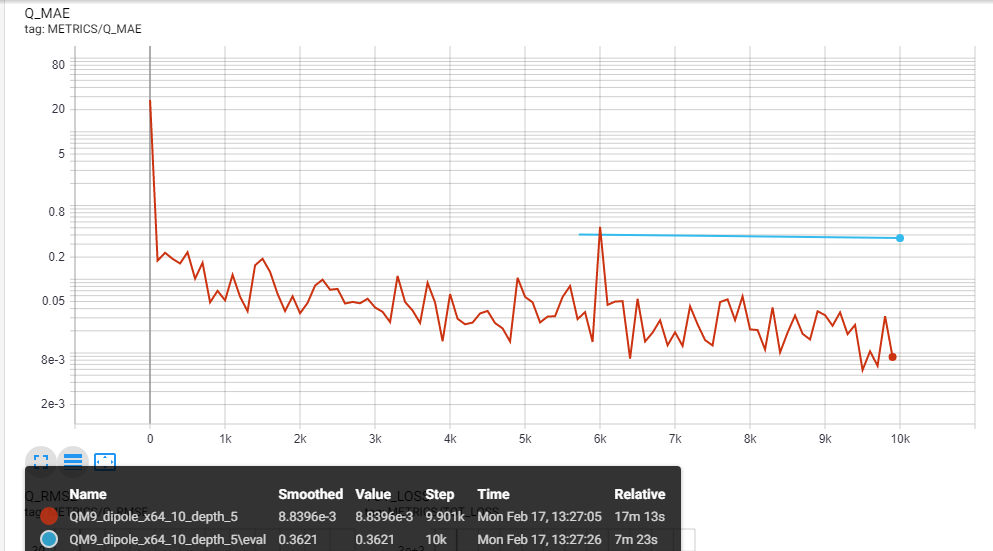
\includegraphics[width=0.85 \textwidth]{C:/Users/hp/Desktop/thesis/Q_MAE_10.png}
\caption{The MAE trend for partial charges regressed against molecular dipole moment upto 10k training steps built using (N=10) QM9 molecules with a training time of 17 minutes}
\end{figure}

\begin{figure} 
\centering
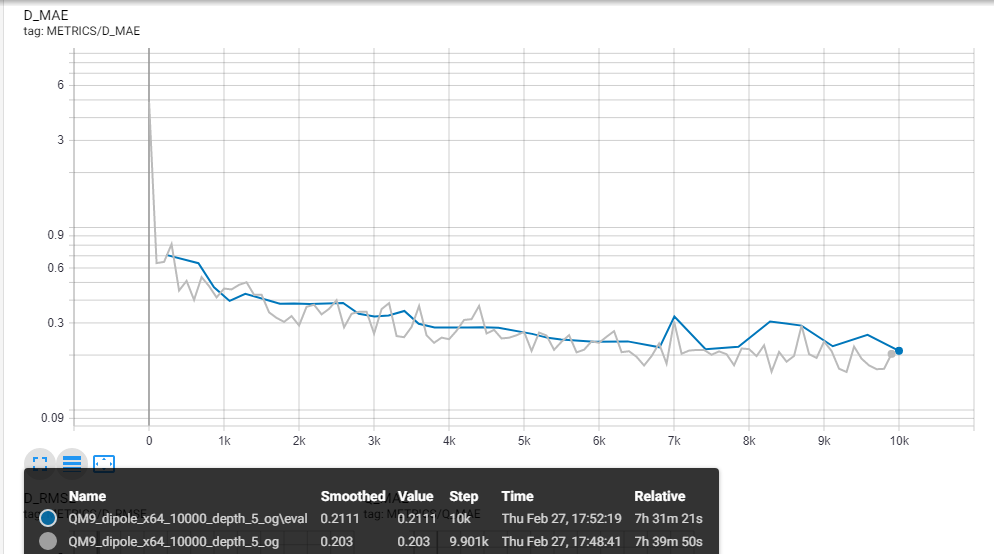
\includegraphics[width=0.85 \textwidth]{C:/Users/hp/Desktop/thesis/D_MAE_10000.png}
\caption{The MAE trend for molecular dipole moment upto 10k training steps built using (N=10000) QM9 molecules with a training time of 7 hours and 40 minutes}
\end{figure}

\begin{figure} [H]
\centering
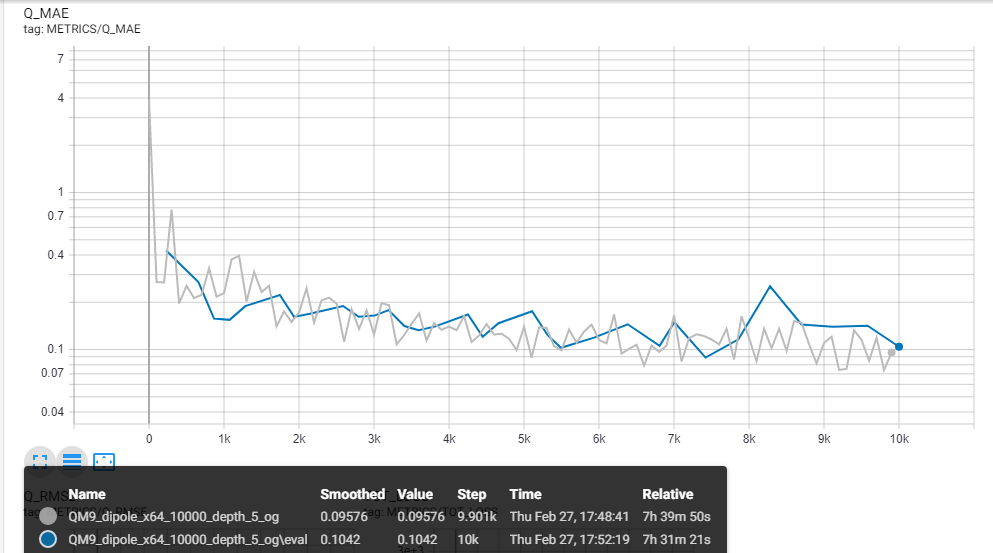
\includegraphics[width=0.85 \textwidth]{C:/Users/hp/Desktop/thesis/Q_MAE_10000.png}
\caption{The MAE trend for partial charges regressed against the molecular dipole moment upto 10k training steps built using (N=10000) QM9 molecules with a training time of 7 hours and 40 minutes}
\end{figure}

\begin{figure} 
\centering
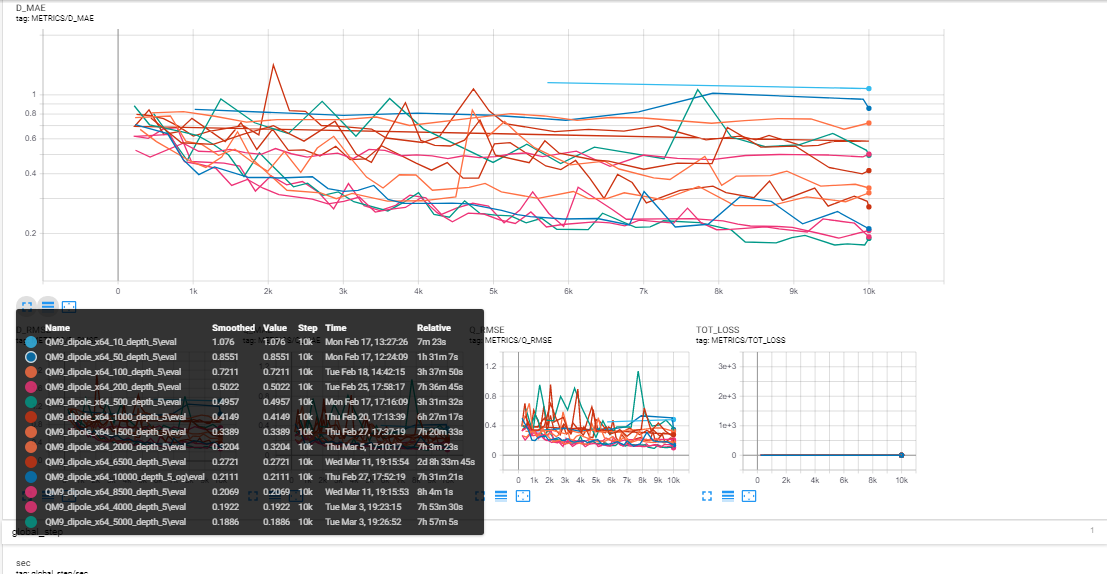
\includegraphics[width=0.85 \textwidth]{C:/Users/hp/Desktop/thesis/D_MAE.png}
\caption{The MAE trend for molecular dipole moment for all the 13 dipole models trained upto 10k training steps built using N=10,50,100,200,500,1000,1500,2000,4000,5000,6500,8500,10000 QM9 molecules}
\label{D_MAE}
\end{figure}

\begin{figure} [H]
\centering
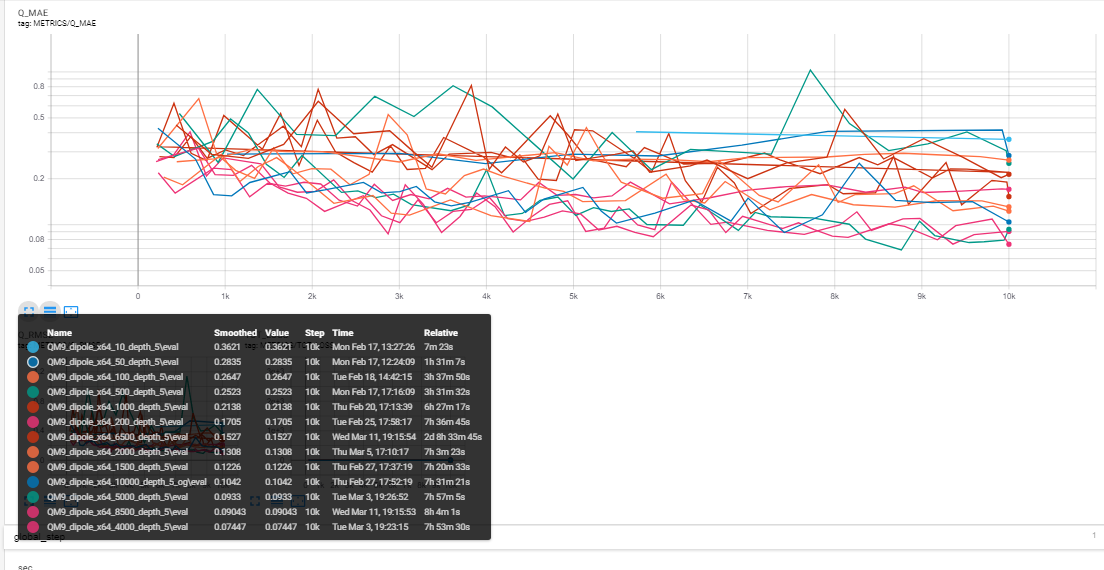
\includegraphics[width=0.85 \textwidth]{C:/Users/hp/Desktop/thesis/Q_MAE.png}
\caption{The MAE trend for partial charges for all the 13 dipole models trained upto 10k training steps built using \linebreak
N=10,50,100,200,500,1000,1500,2000,4000,5000,6500,8500,10000 QM9 molecules}
\label{Q_MAE}
\end{figure}
The Figures \ref{D_MAE} and \ref{Q_MAE} both show \emph{the decreasing trend of the MAE values} for all the 13 dipole models using N QM9 molecules built with various sample training sizes. It is apparent that increasing the training sample size, decreases the MAE value causing the dipole model to be more accurate in this trend. For the purpose of testing the ANNs with different training sample sizes, we focus on the final MAE value at the last training step.

\begin{figure} [H]
\centering
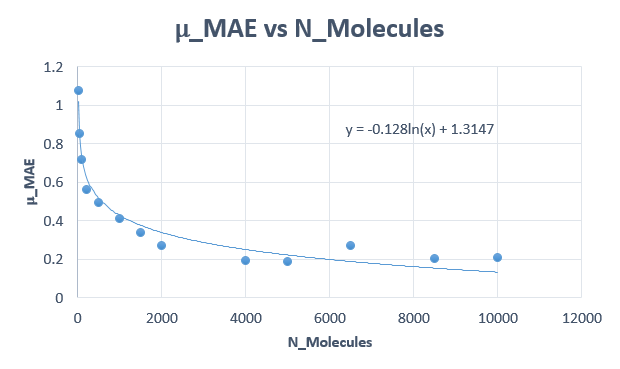
\includegraphics[width=0.85 \textwidth]{C:/Users/hp/Desktop/thesis/MAE_Log.png}
\caption{The Logarithmic trend for the MAE of molecular dipole moment $\mu$ at 10k training steps built using \linebreak
N=10,50,100,200,500,1000,1500,2000,4000,5000,6500,8500,10000 QM9 molecules}
\end{figure}
\begin{figure} [H]
\centering
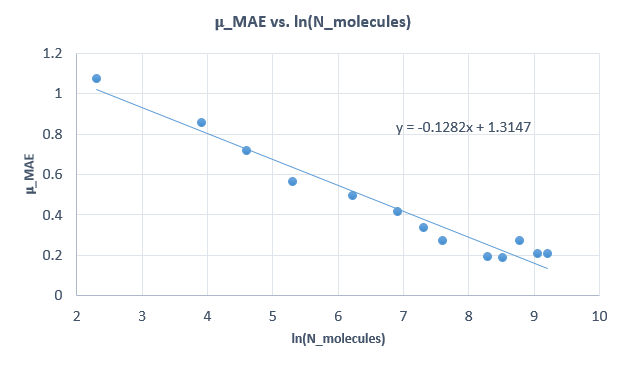
\includegraphics[width=0.85 \textwidth]{C:/Users/hp/Desktop/thesis/MAE_Semi_log.png}
\caption{The Semi-Logarithmic trend for the MAE of molecular dipole moment $\mu$ at 10k training steps built using \linebreak
N=10,50,100,200,500,1000,1500,2000,4000,5000,6500,8500,10000 QM9 molecules gives a slope value of -0.128}
\end{figure}


 The Logarithmic trend follows the equation,

 $\mu_{MAE}=-0.128 ln(N)+1.3147$. This equation for the logarithmic trend in error values can be used as an indicator for the number of molecules $N$ required for training set to predict the molecular dipole moment  $\mu$ with an expected accuracy.


\chapter{Conclusions}
Using the PiNN - Python Library for building Atomic Neural Networks for molecules and materials, a quantitative structure-property relation was established for the molecular dipole moment of a database of molecules (QM9 Dataset).

Molecular dipole moment is predicted using PiNet with different training sizes and their accuracies are compared with exact values. The result showed that the error decreases with the increasing number of trained molecules which follows the logarithmic trend. 

The result showed the logarithmic trend in error values which can be used as an indicator for number molecules required for training set to predict the molecular dipole moment with an expected accuracy. Thus, building ANNs with improved accuracy and minimizing computational time.

\begin{thebibliography}{100}
\bibitem{QM} Dirac, P. A. M. \emph{Quantum mechanics of many-electron systems.} Proc. R. Soc. London, Ser. A 1929, 123, 714–733.
\bibitem{ML} Michael A. Nielsen, \emph{Neural Networks and Deep Learning}, Determination Press 2015.
\bibitem{simANN} Butler, K. T.; Davies, D. W.; Cartwright, H.; Isayev, O.; Walsh, A. \emph{Machine learning for molecular and materials science.} Nature 2018, 559, 1–9.
\bibitem{BPNN} Behler, J.; Parrinello, M. \emph{Generalized Neural-Network Representation of High-Dimensional Potential-Energy Surfaces.} Phys. Rev. Lett. 2007, 98, 146401.
\bibitem{atmfing} Duvenaud, D. Maclaurin, D. Aguilera-Iparraguirre, J. Gómez-Bombarelli, R.Hirzel, T. i. Aspuru-Guzik, A.Adams, R. P. \emph{Convolutional networks on graphs for learning molecular fingerprints.} Adv. Neural Inf. Process. Syst. 2015; pp 2224–2232.
\bibitem{GCNN} Schütt, K. T. Arbabzadah, F.Chmiela, S. Müller, K. R.Tkatchenko, A. \emph{Quantum-chemical insights from deep tensor neural networks.} Nat. Commun. 2017, 8, 13890.
\bibitem{fthier} Lubbers, N.; Smith, J. S.; Barros, K. \emph{Hierarchical modeling of molecular energies using a deep neural network.} J. Chem. Phys. 2018, 148, 241715.
\bibitem{PiNN} Yunqi Shao,  Matti Hellström,  Pavlin D. Mitev, Lisanne Knijff, and Chao Zhang, \emph{PiNN: A Python Library for Building Atomic Neural Networks of Molecules and Materials.} arXiv:1910.03376v1 [physics.comp-ph] 8 Oct 2019
\bibitem{msg} Behler, J. \emph{Constructing High-Dimensional Neural Network Potentials: A Tutorial Review.} Int. J. Quantum Chem. 2015, 115, 1032–1050.
\bibitem{tf} Abadi, M.; Agarwal, A.; Barham, P.; Brevdo, E.; Chen, Z.; Citro, C.; Corrado, G. S.; Davis, A.; Dean, J.; Devin, M.; Ghemawat, S.; Goodfellow, I.; Harp, A.; Irving, G.; Isard, M.; Jia, Y.; Jozefowicz, R.; Kaiser, L.; Kudlur, M.; Levenberg, J.; Mane, D.; Monga, R.; Moore, S.; Murray, D.; Olah, C.; Schuster, M.; Shlens, J.; Steiner, B.; Sutskever, I.; Talwar, K.; Tucker, P.; Vanhoucke, V.; Vasudevan, V.; Viegas, F.; Vinyals, O.; Warden, P.; Wattenberg, M.; Wicke, M.; Yu, Y.; Zheng, X. \emph{TensorFlow: Large-Scale Machine Learning on Heterogeneous Distributed Systems.} 2016.
\bibitem{QM9} Ramakrishnan, R.; Dral, P. O.; Rupp, M.; Von Lilienfeld, O. A. \emph{Quantum chemistry structures and properties of 134 kilo molecules.} Sci. Data 2014, 1, 140022.
\bibitem{DFT} Becke, A. D. \emph{Density-functional thermochemistry. III. The role of exact exchange.} J. Chem. Phys. 1993, 98, 5648–5652.

\end{thebibliography}
\end{document} 